\chapter{Re 5000 Time Averaged Fields}
\label{app: RE5000}
\begin{figure}[htbp]
  \centering
  \setlength{\tabcolsep}{0pt}
  \captionsetup[subfigure]{skip=1pt}

  % --- column headers ---
  \makebox[0.32\textwidth]{$\mathcal{S}$}
  \makebox[0.32\textwidth]{$\mathcal{S}_\text{ref}$}
  \makebox[0.32\textwidth]{$\bigl| \mathcal{S}-\mathcal{S}_\text{ref}\bigr|$}\par
  \vspace{1pt}

  % --- row 1: <u'u'> ---
  \rotatebox{90}{\makebox[0.30\textwidth][c]{$\langle u'u'\rangle$}}%
  \begin{subfigure}[t]{0.3\textwidth}
    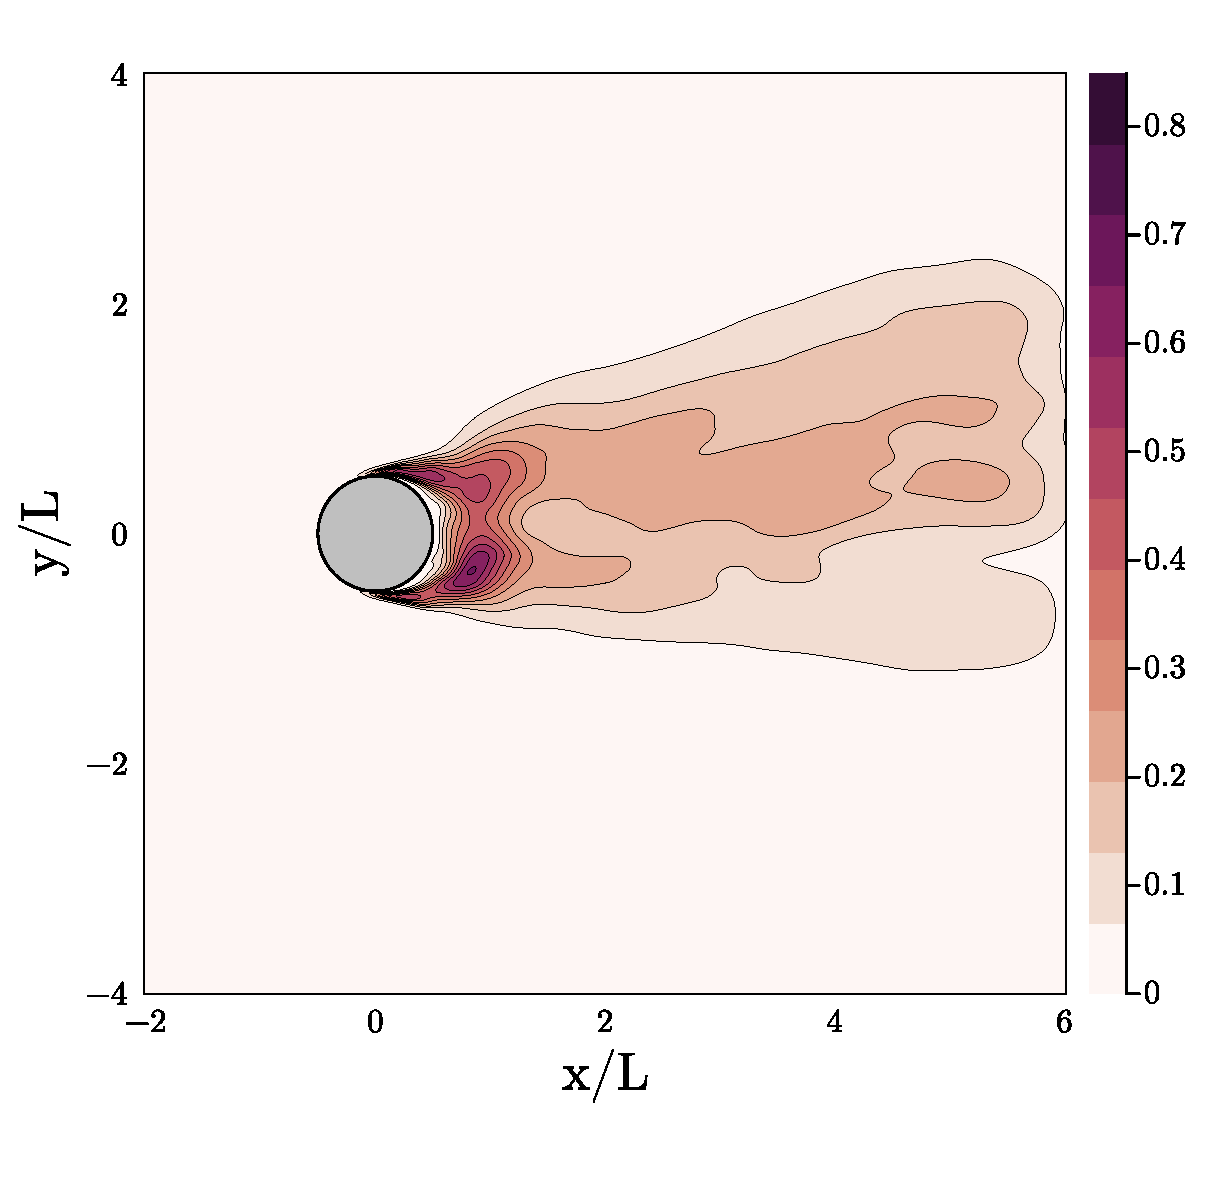
\includegraphics[width=\linewidth]{figures/Results/RE5000/rst_panels/rst_uu_hybrid.pdf}
    % \caption{}
    \label{fig: RE5000_rst_uu_hybrid}
  \end{subfigure}
  \begin{subfigure}[t]{0.3\textwidth}
    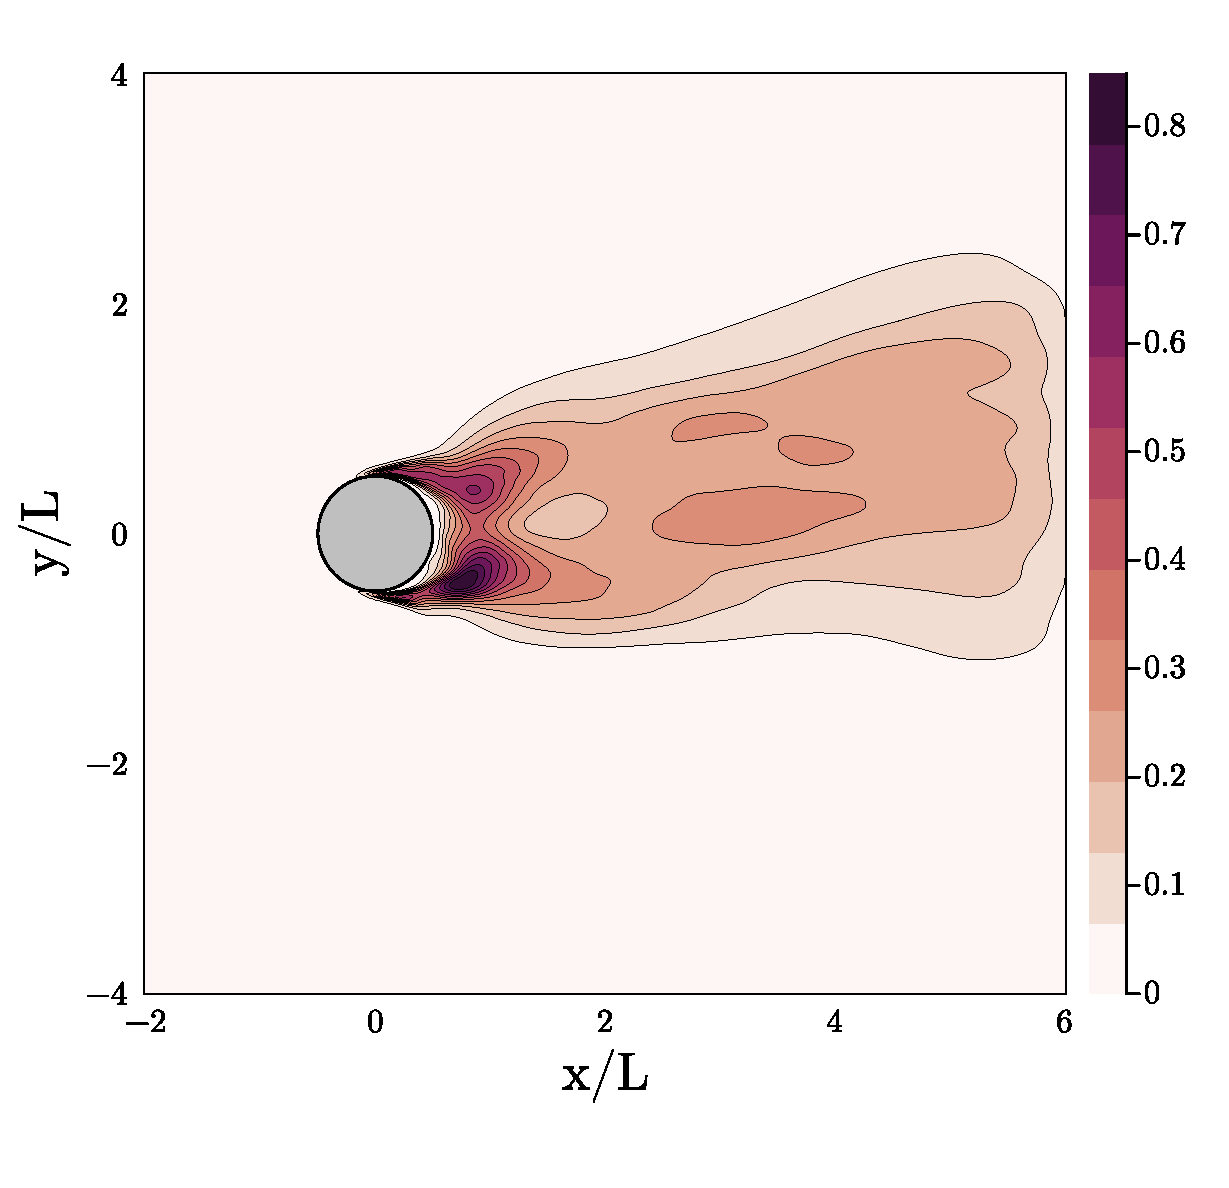
\includegraphics[width=\linewidth]{figures/Results/RE5000/rst_panels/rst_uu_reference.pdf}
    % \caption{}
    \label{fig: RE5000_rst_uu_ref}
  \end{subfigure}
  \begin{subfigure}[t]{0.3\textwidth}
    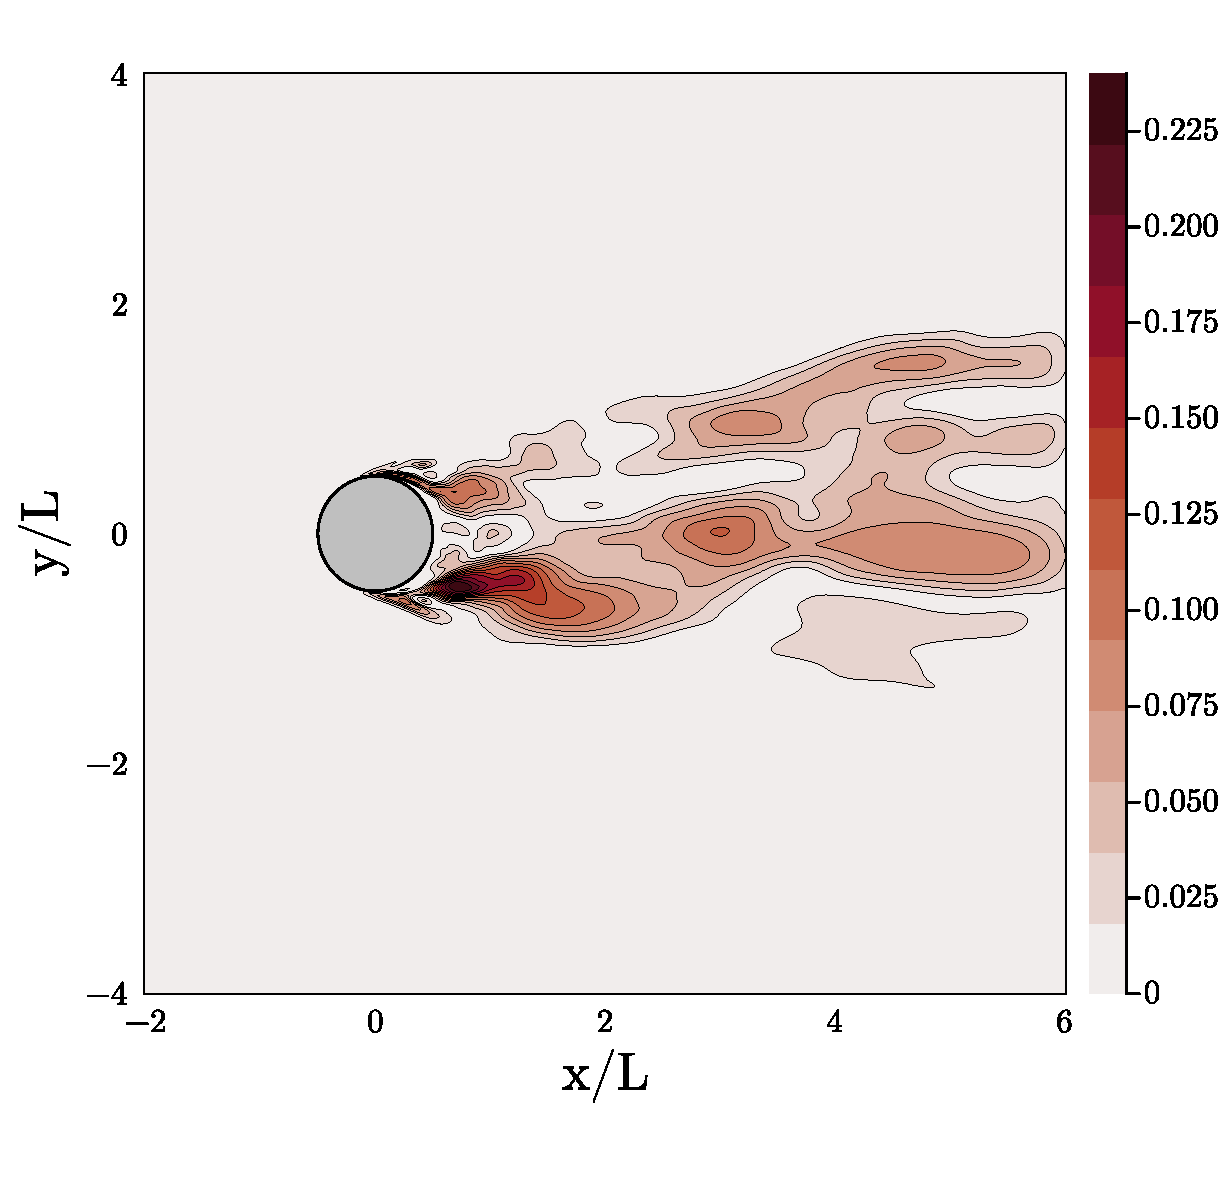
\includegraphics[width=\linewidth]{figures/Results/RE5000/rst_panels/rst_uu_abserror.pdf}
    % \caption{}
    \label{fig: RE5000_rst_uu_diff}
  \end{subfigure}

  \vspace{-2em}

  % --- row 2: <v'v'> ---
  \rotatebox{90}{\makebox[0.30\textwidth][c]{$\langle v'v'\rangle$}}%
  \begin{subfigure}[t]{0.3\textwidth}
    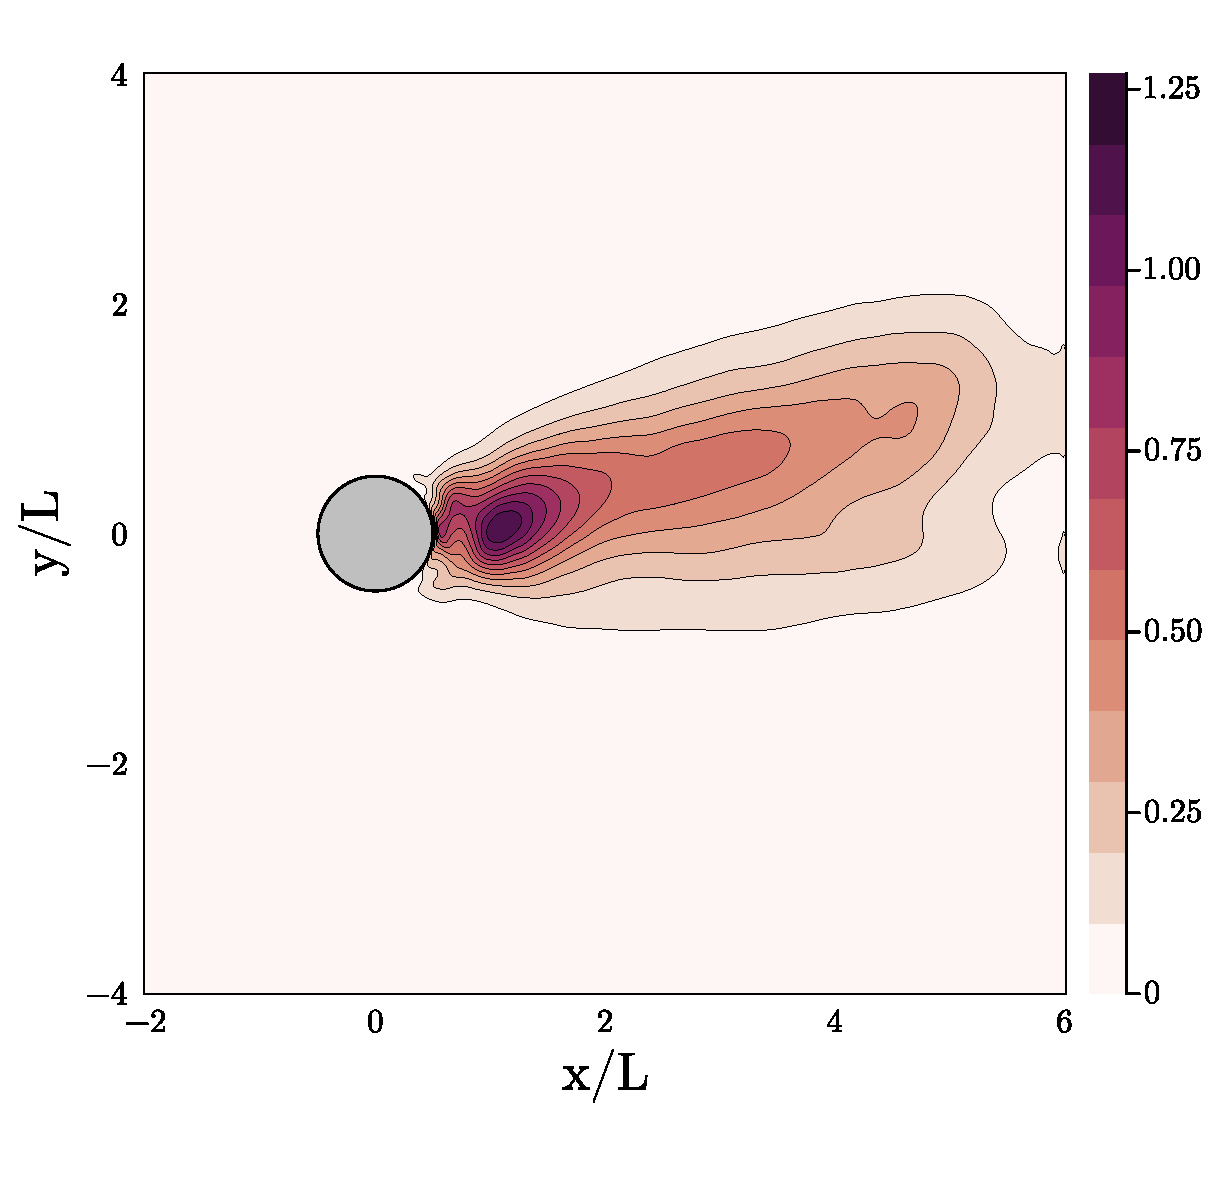
\includegraphics[width=\linewidth]{figures/Results/RE5000/rst_panels/rst_vv_hybrid.pdf}
    % \caption{}
    \label{fig: RE5000_rst_vv_hybrid}
  \end{subfigure}
  \begin{subfigure}[t]{0.3\textwidth}
    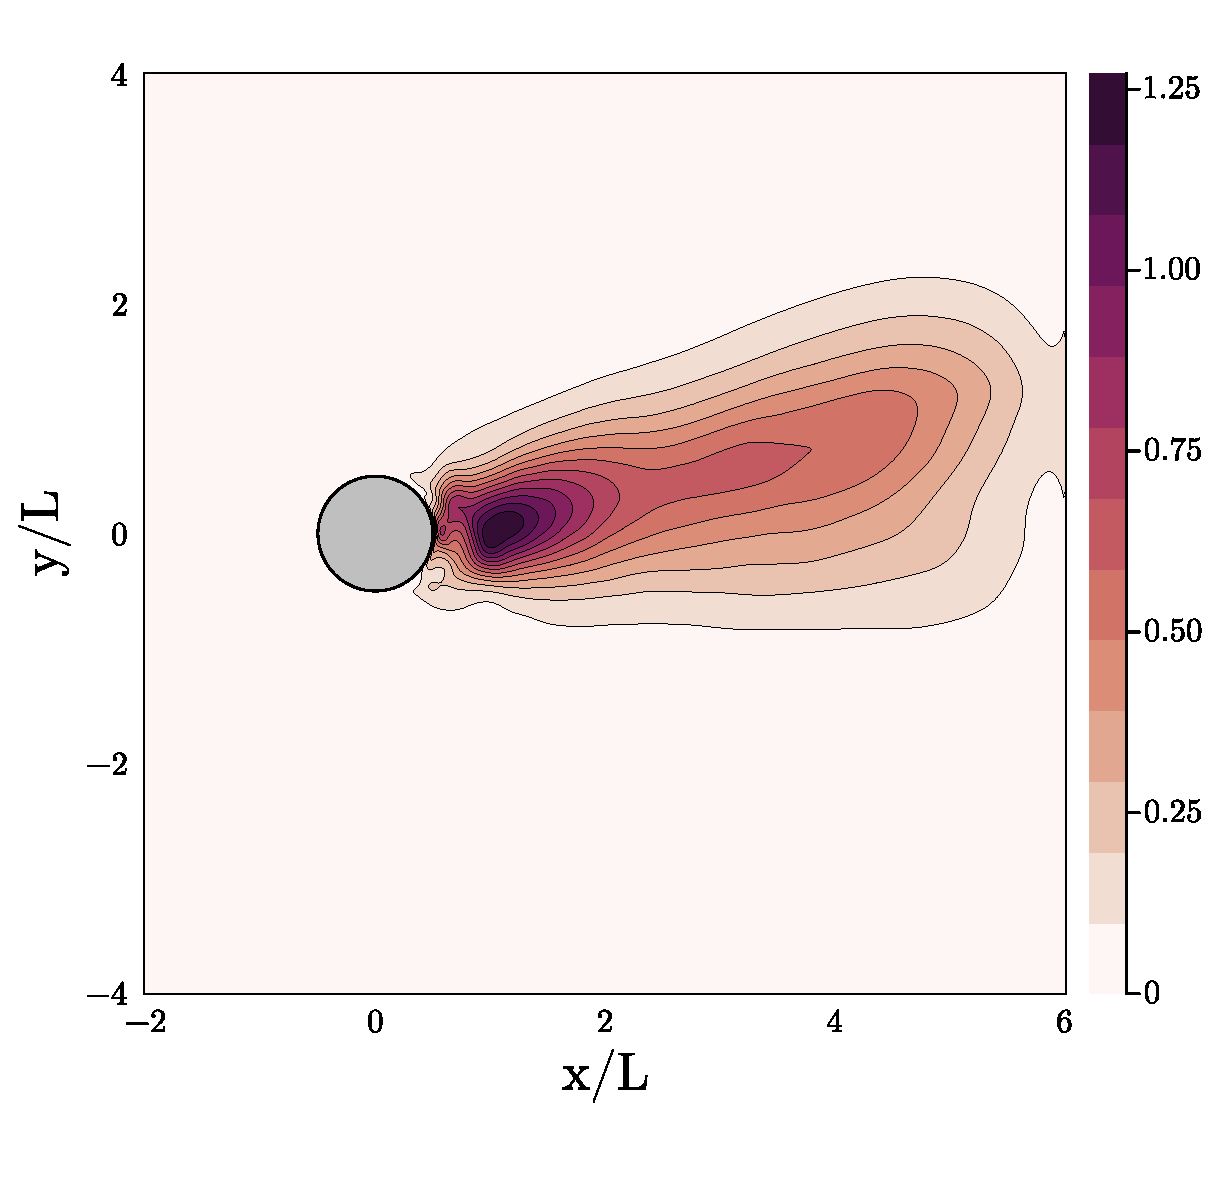
\includegraphics[width=\linewidth]{figures/Results/RE5000/rst_panels/rst_vv_reference.pdf}
    % \caption{}
    \label{fig: RE5000_rst_vv_ref}
  \end{subfigure}
  \begin{subfigure}[t]{0.3\textwidth}
    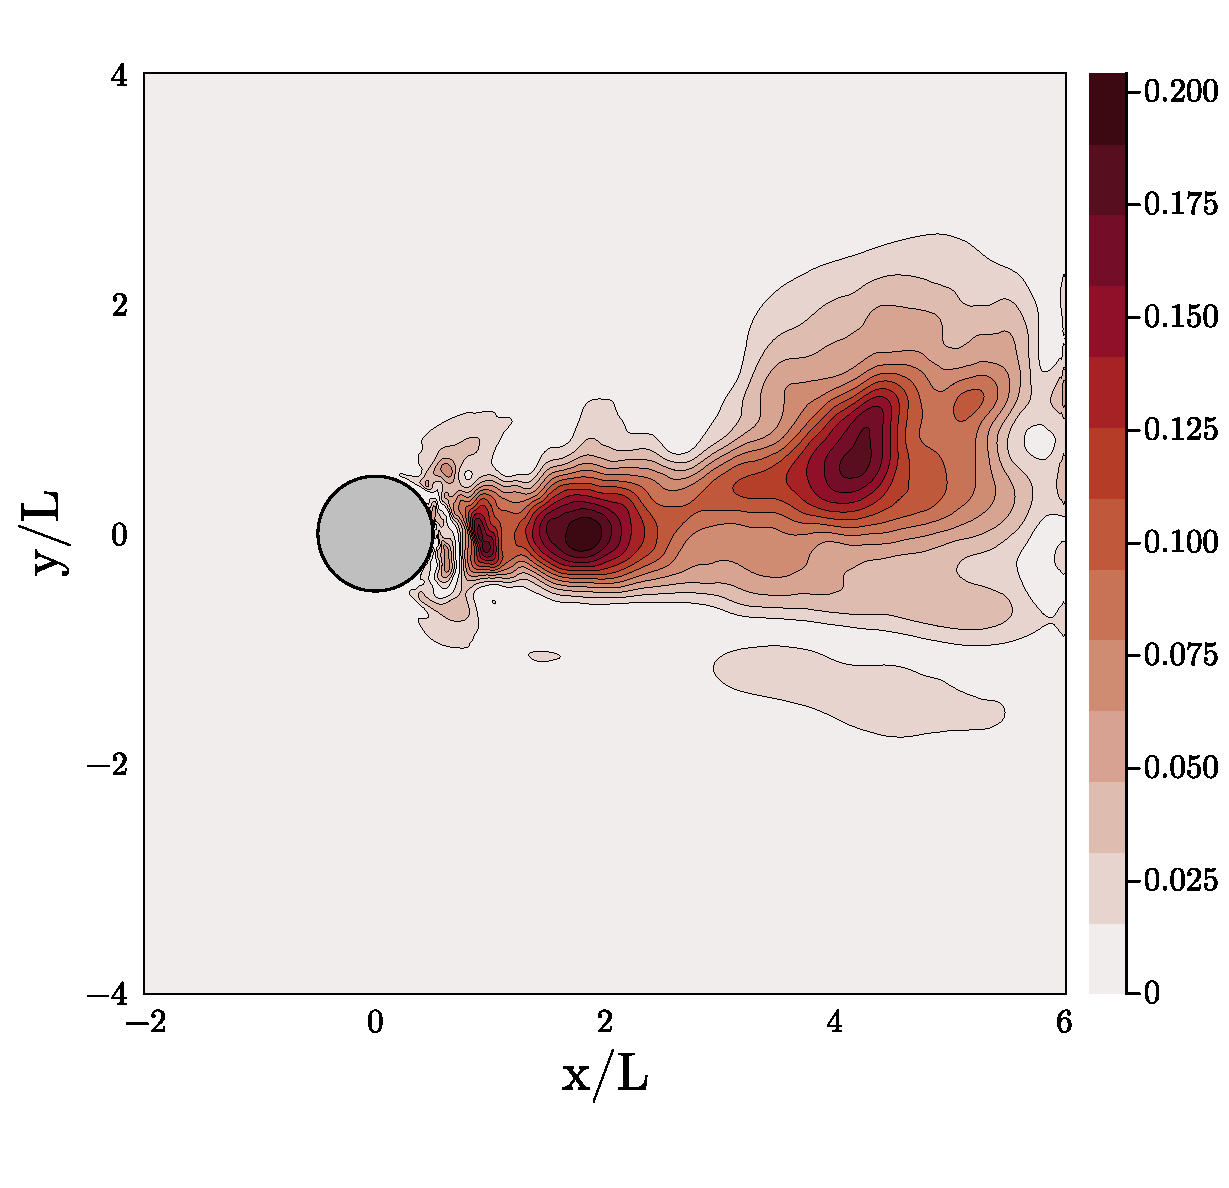
\includegraphics[width=\linewidth]{figures/Results/RE5000/rst_panels/rst_vv_abserror.pdf}
    % \caption{}
    \label{fig: RE5000_rst_vv_diff}
  \end{subfigure}

  \vspace{-2em}

  % --- row 3: <u'v'> ---
  \rotatebox{90}{\makebox[0.30\textwidth][c]{$\langle u'v'\rangle$}}%
  \begin{subfigure}[t]{0.3\textwidth}
    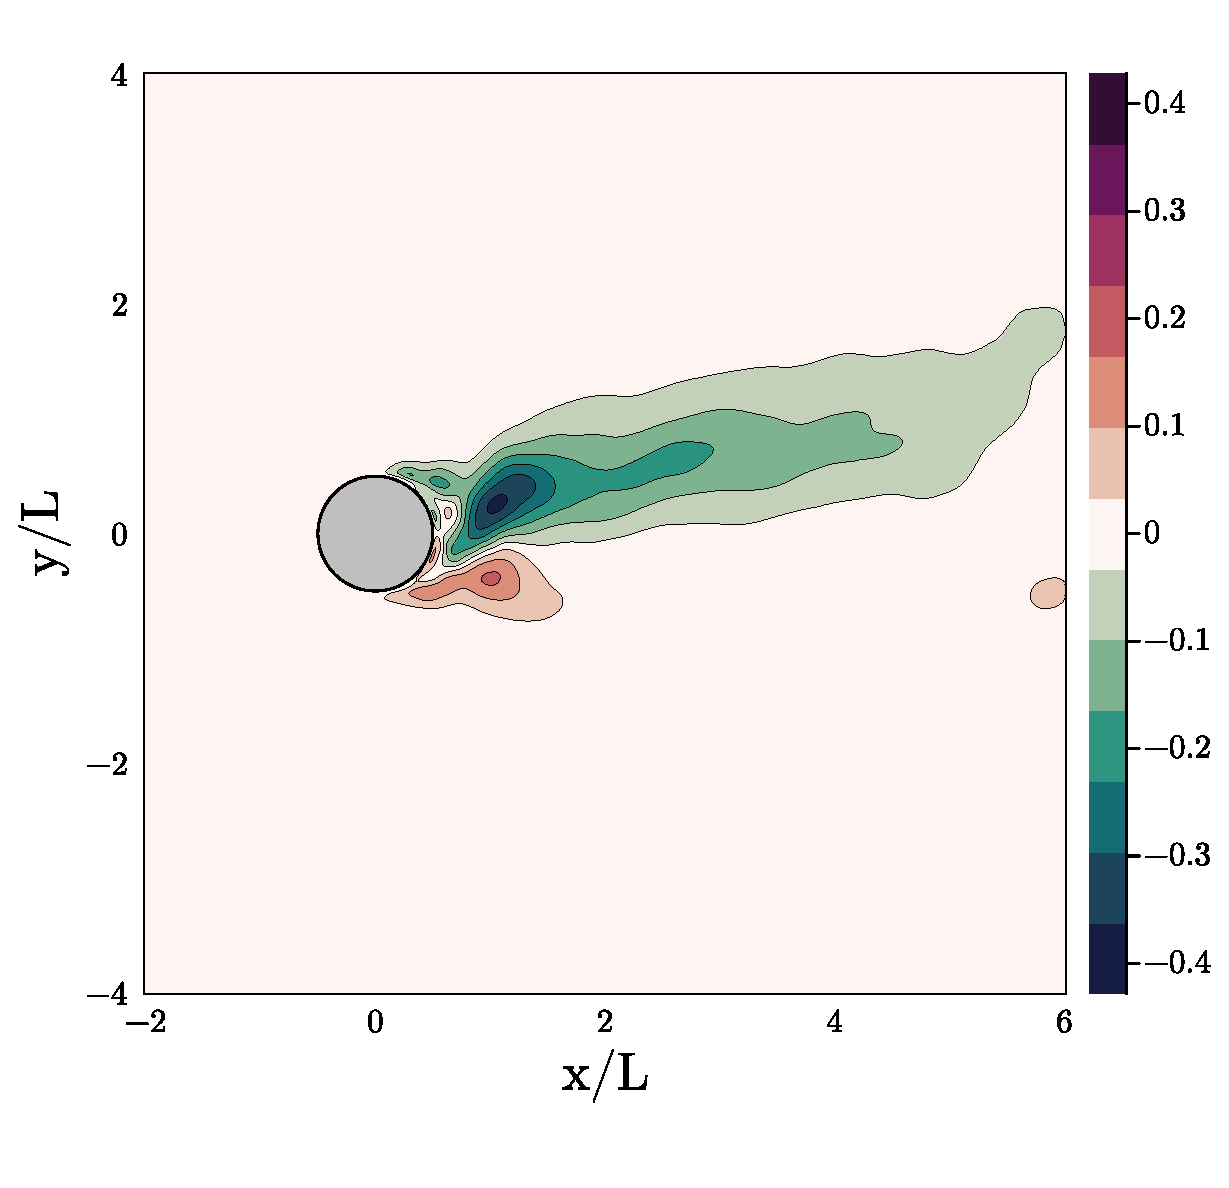
\includegraphics[width=\linewidth]{figures/Results/RE5000/rst_panels/rst_uv_hybrid.pdf}
    % \caption{}
    \label{fig: RE5000_rst_uv_hybrid}
  \end{subfigure}
  \begin{subfigure}[t]{0.3\textwidth}
    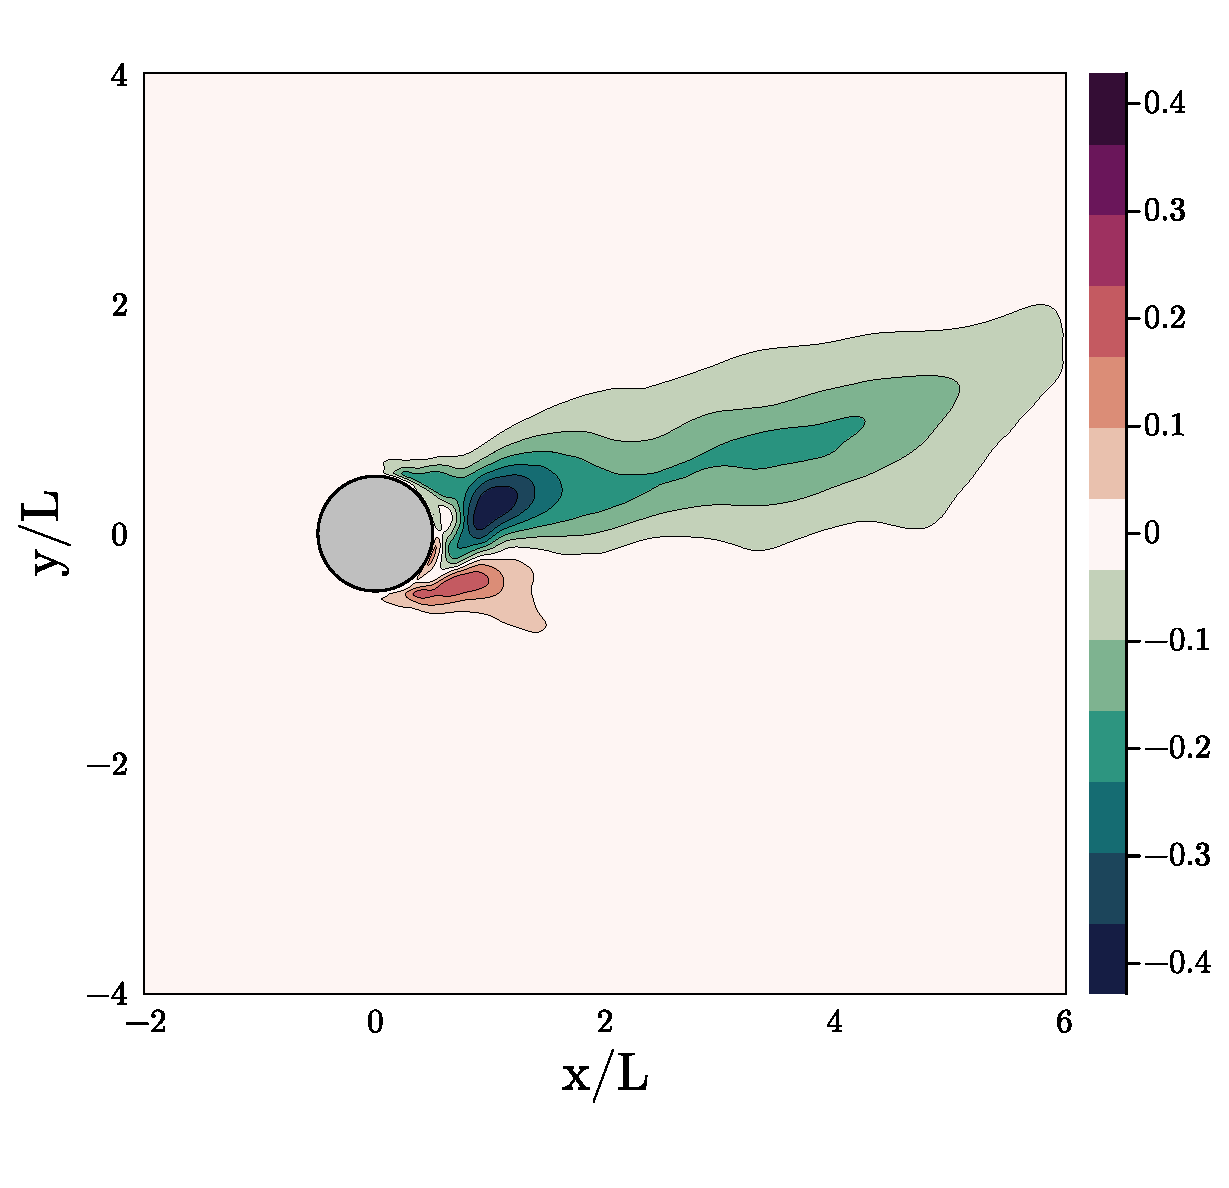
\includegraphics[width=\linewidth]{figures/Results/RE5000/rst_panels/rst_uv_reference.pdf}
    % \caption{}
    \label{fig: RE5000_rst_uv_ref}
  \end{subfigure}
  \begin{subfigure}[t]{0.3\textwidth}
    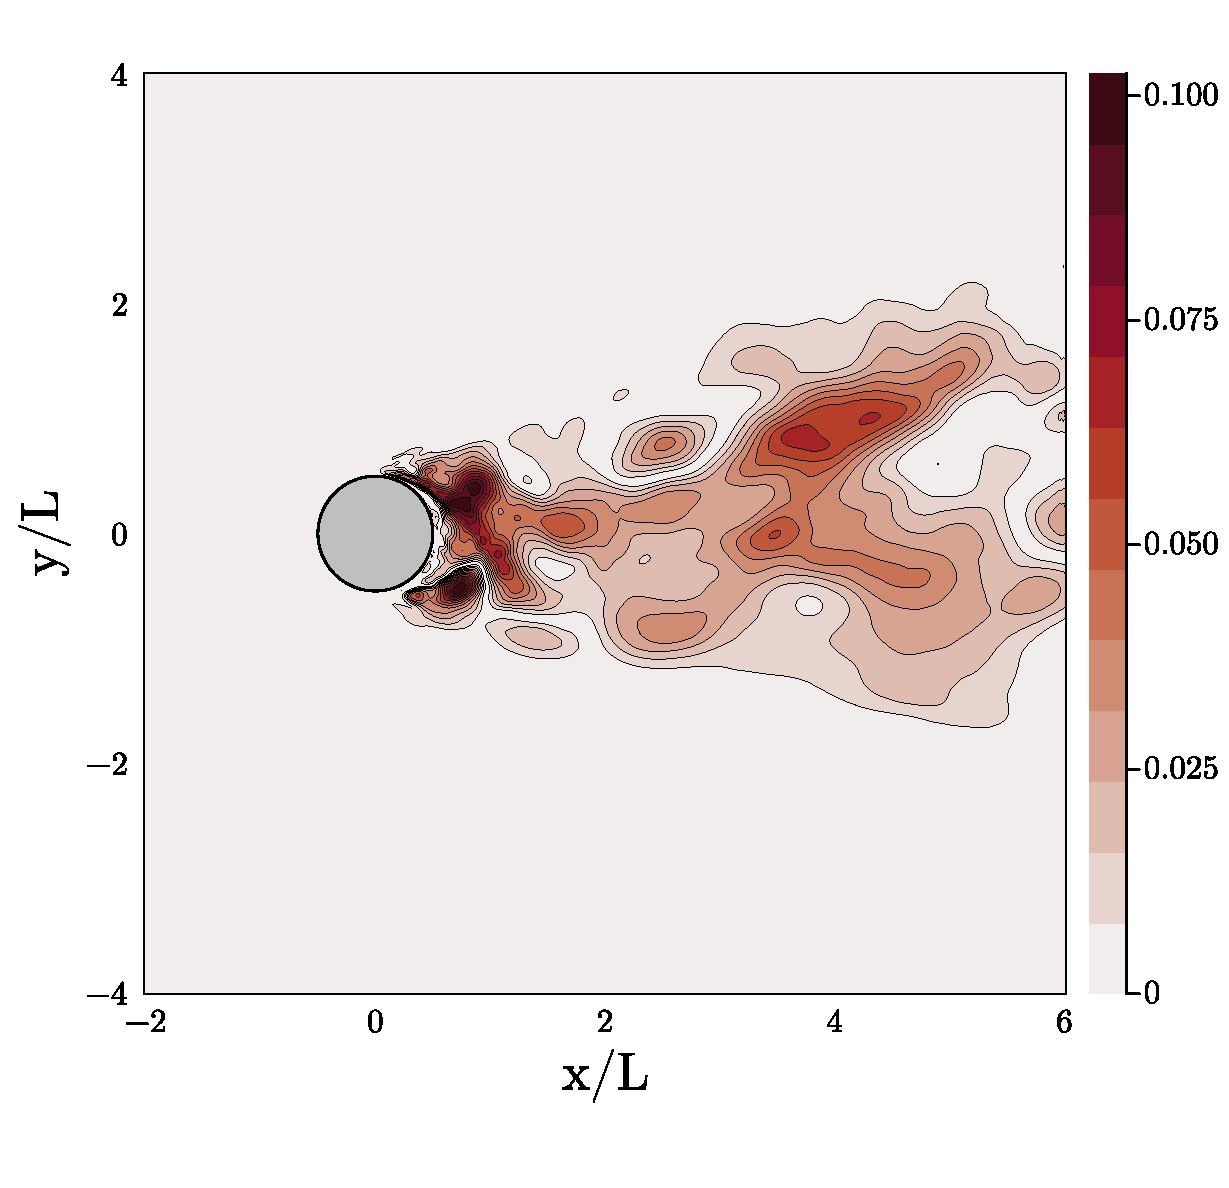
\includegraphics[width=\linewidth]{figures/Results/RE5000/rst_panels/rst_uv_abserror.pdf}
    % \caption{}
    \label{fig: RE5000_rst_uv_diff}
  \end{subfigure}
\vspace{-2em}
\caption{Time-averaged Reynolds-stress components at $Re=5000$, top to bottom $\langle u'u'\rangle$, $\langle v'v'\rangle$, $\langle u'v'\rangle$. Columns: hybrid estimate $\mathcal{S}$, reference solver $\mathcal{S}_\text{ref}$, and absolute difference $\bigl|\mathcal{S}-\mathcal{S}_\text{ref}\bigr|$. The hybrid recovers the spatial structure of each component, with residuals concentrated in the energetic near wake. Lengths scaled by $L$, velocities by $U$.}
\label{fig: RE5000_rst}
\end{figure}


\begin{figure}[htbp]
  \centering
  \setlength{\tabcolsep}{0pt}        % no inter-column padding if you switch to tabular
  \captionsetup[subfigure]{skip=1pt} % shrink gap between image and subcaption

    \makebox[0.32\textwidth]{$\mathcal{S}$}
  \makebox[0.32\textwidth]{$\mathcal{S}_\text{ref}$}
  \makebox[0.32\textwidth]{$\bigl| \mathcal{S}-\mathcal{S}_\text{ref}\bigr|$}\par
  \vspace{1pt}
  % --- row 1 ---
    \rotatebox{90}{\makebox[0.33\textwidth][c]{$\langle u\rangle$}}%
  \begin{subfigure}[t]{0.32\textwidth}
    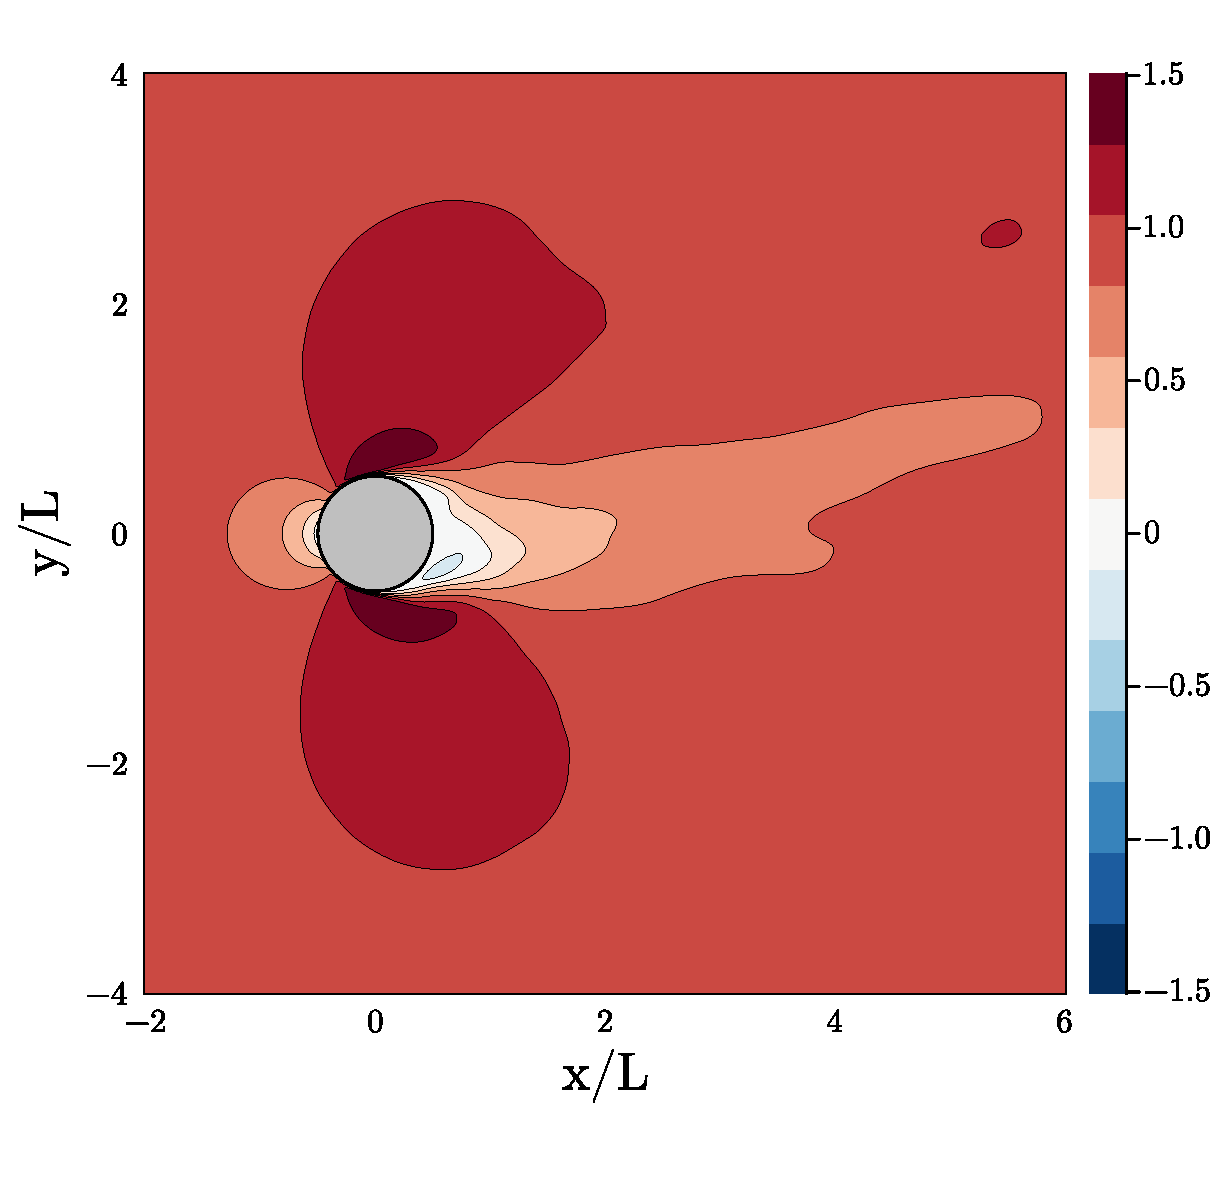
\includegraphics[width=\linewidth]{figures/Results/RE5000/meanflow_panels/meanflow_u_hybrid.pdf}
    \caption{}
    \label{fig: RE5000_hybrid_mean_u}
  \end{subfigure}\hfill
  \begin{subfigure}[t]{0.32\textwidth}
    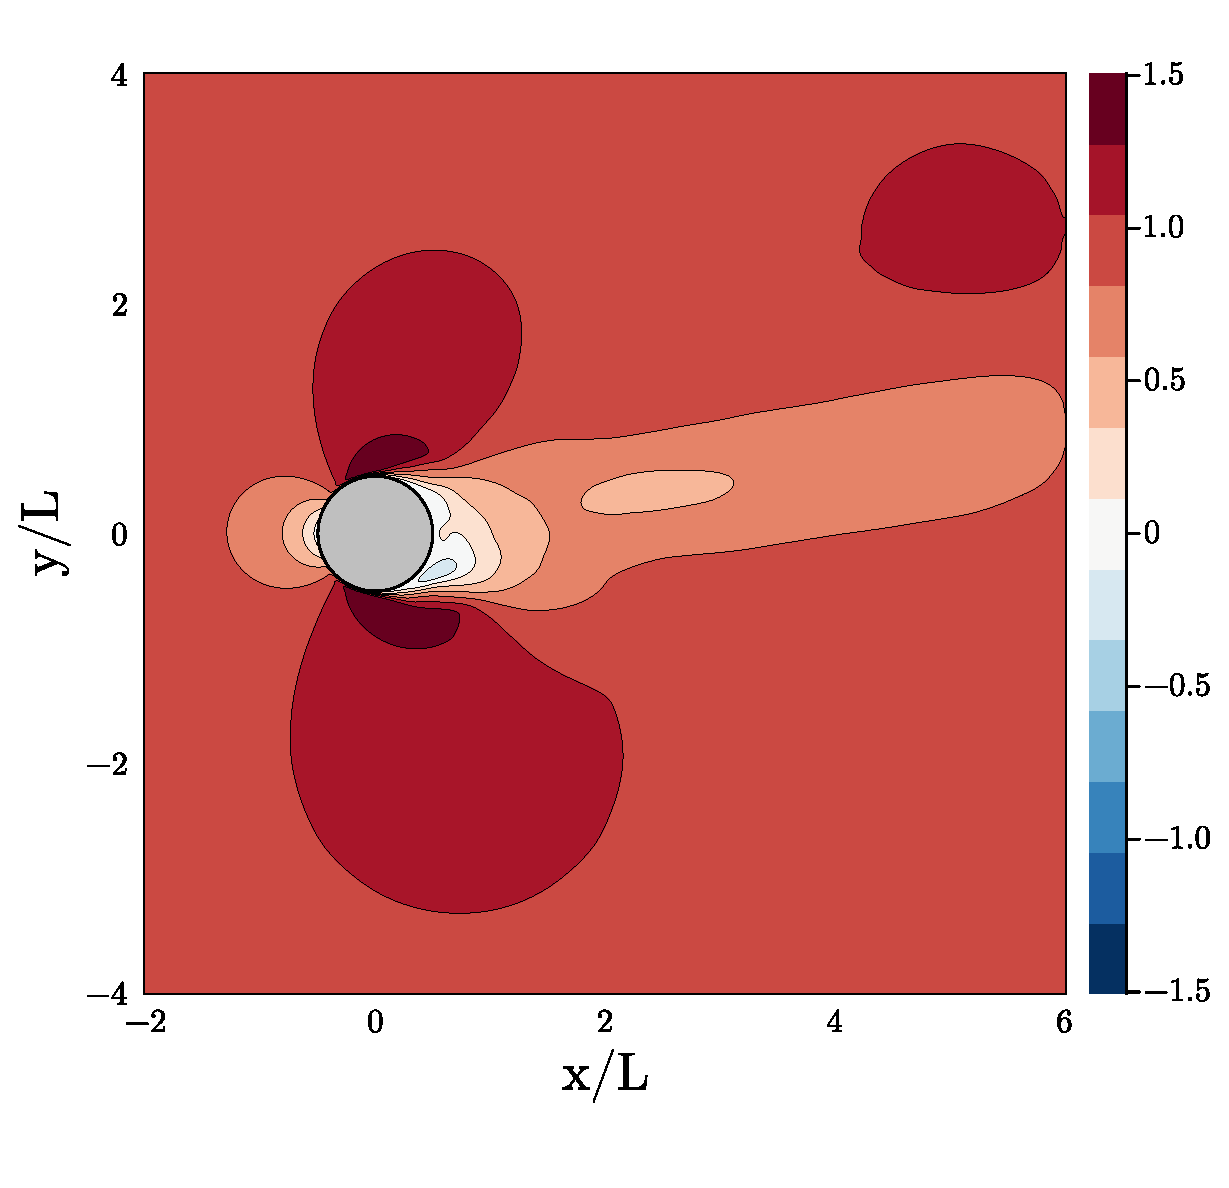
\includegraphics[width=\linewidth]{figures/Results/RE5000/meanflow_panels/meanflow_u_reference.pdf}
    \caption{}
    \label{fig: RE5000_ref_mean_u}
  \end{subfigure}\hfill
  \begin{subfigure}[t]{0.32\textwidth}
    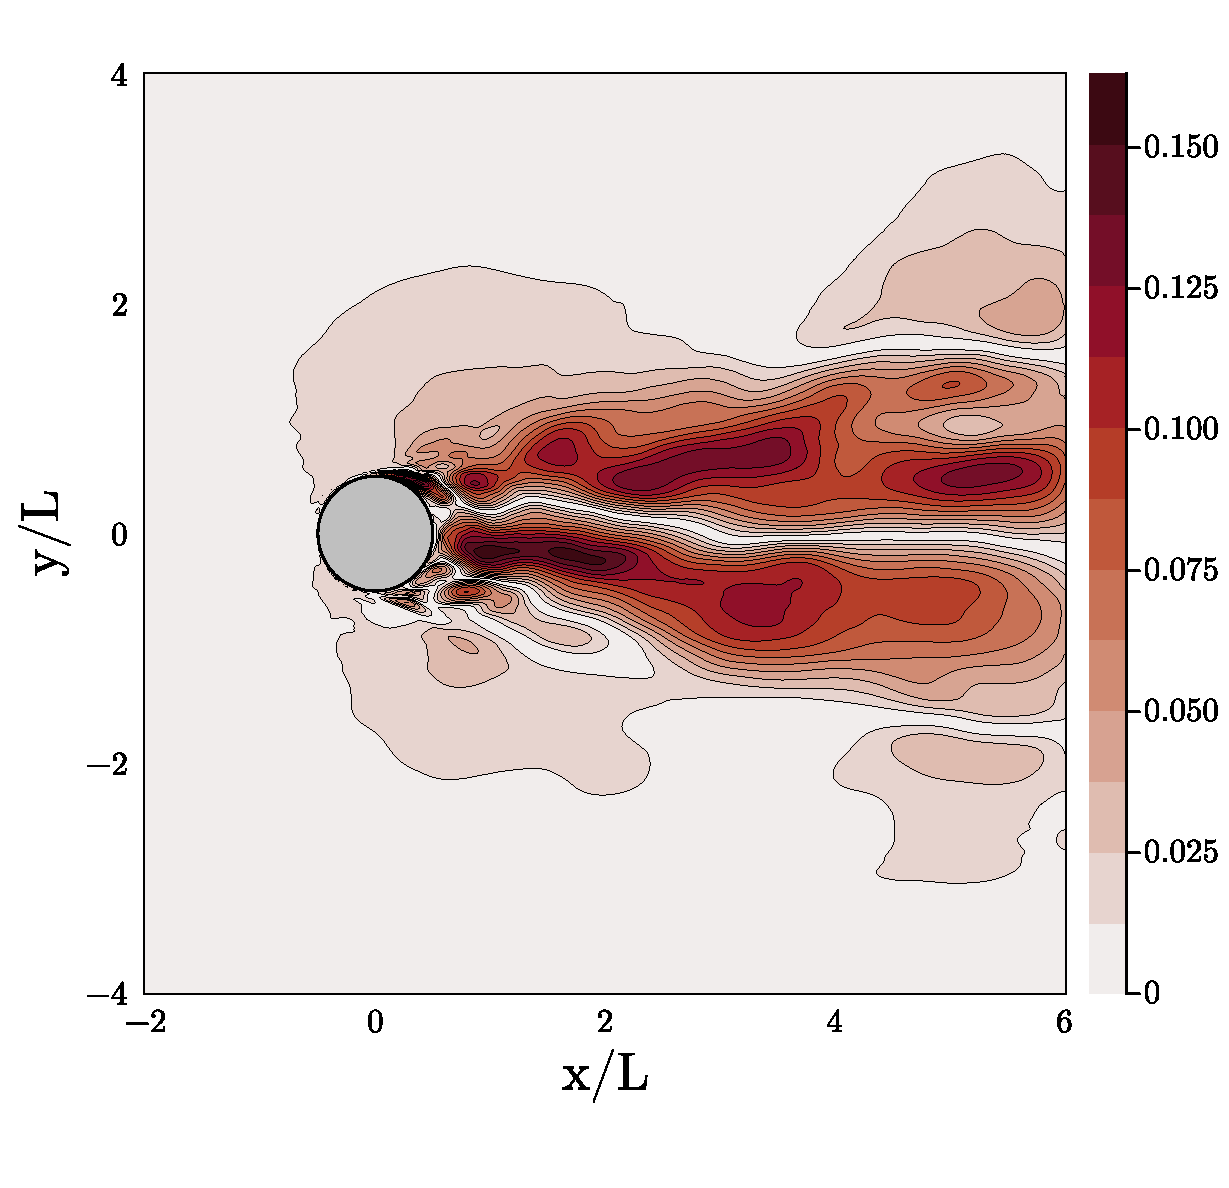
\includegraphics[width=\linewidth]{figures/Results/RE5000/meanflow_panels/meanflow_u_abserror.pdf}
    \caption{}
    \label{fig: RE5000_diff_mean_u}
  \end{subfigure}

  \vspace{-1em} % vertical gap between the two rows; set to 0pt for maximal tightness

  % --- row 2 ---
\rotatebox{90}{\makebox[0.33\textwidth][c]{$\langle v\rangle$}}%
  \begin{subfigure}[t]{0.32\textwidth}
    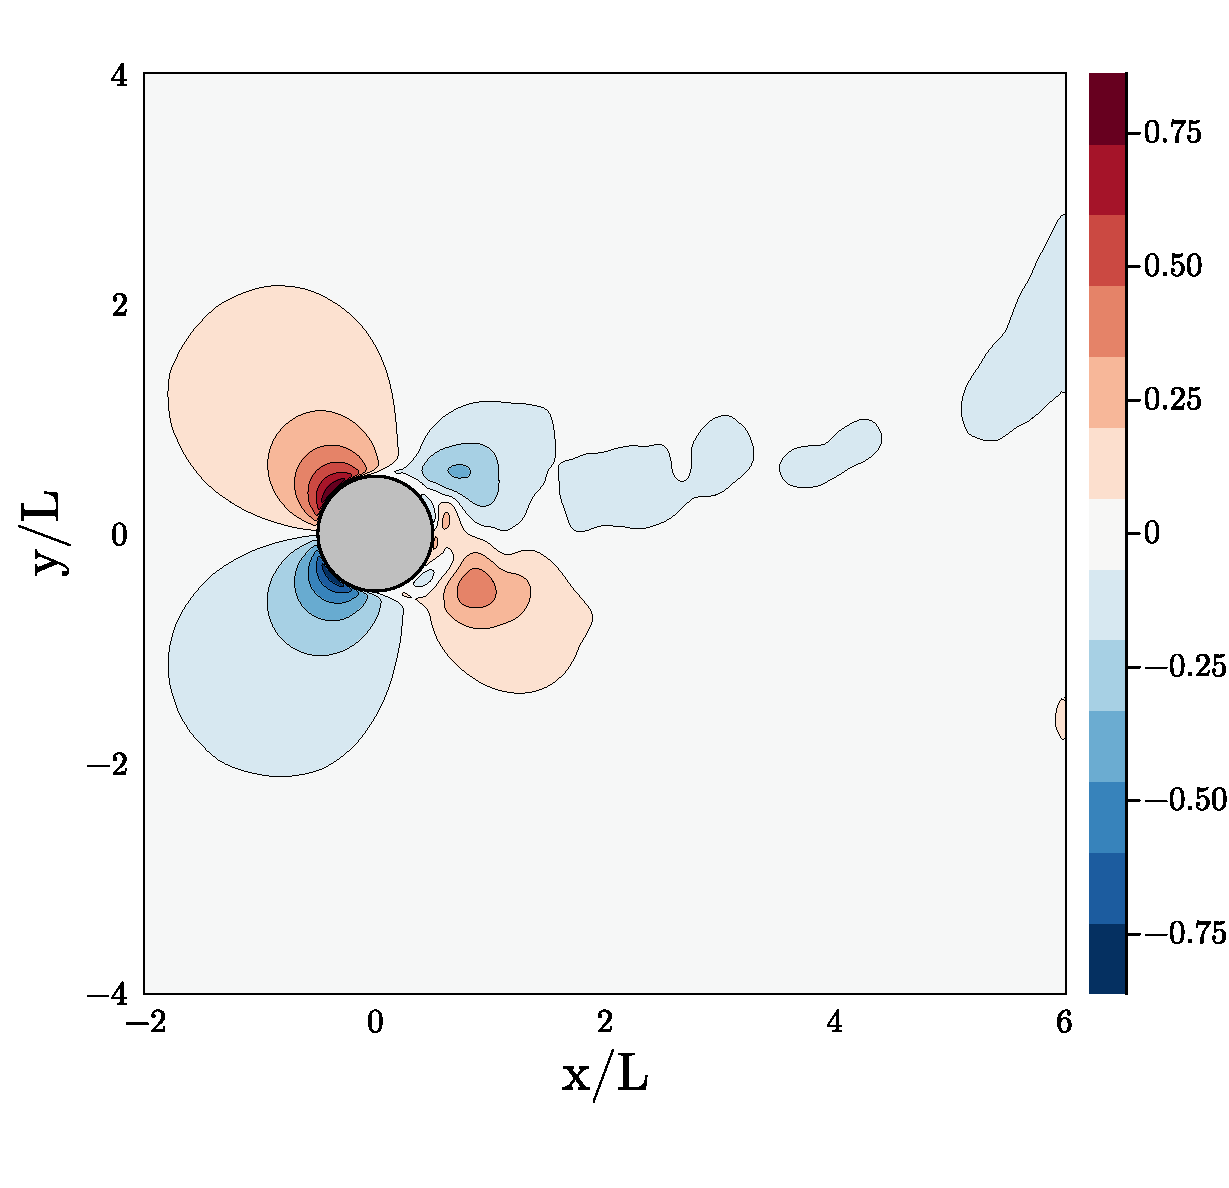
\includegraphics[width=\linewidth]{figures/Results/RE5000/meanflow_panels/meanflow_v_hybrid.pdf}
    \caption{}
    \label{fig: RE5000_hybrid_mean_v}
  \end{subfigure}\hfill
  \begin{subfigure}[t]{0.32\textwidth}
    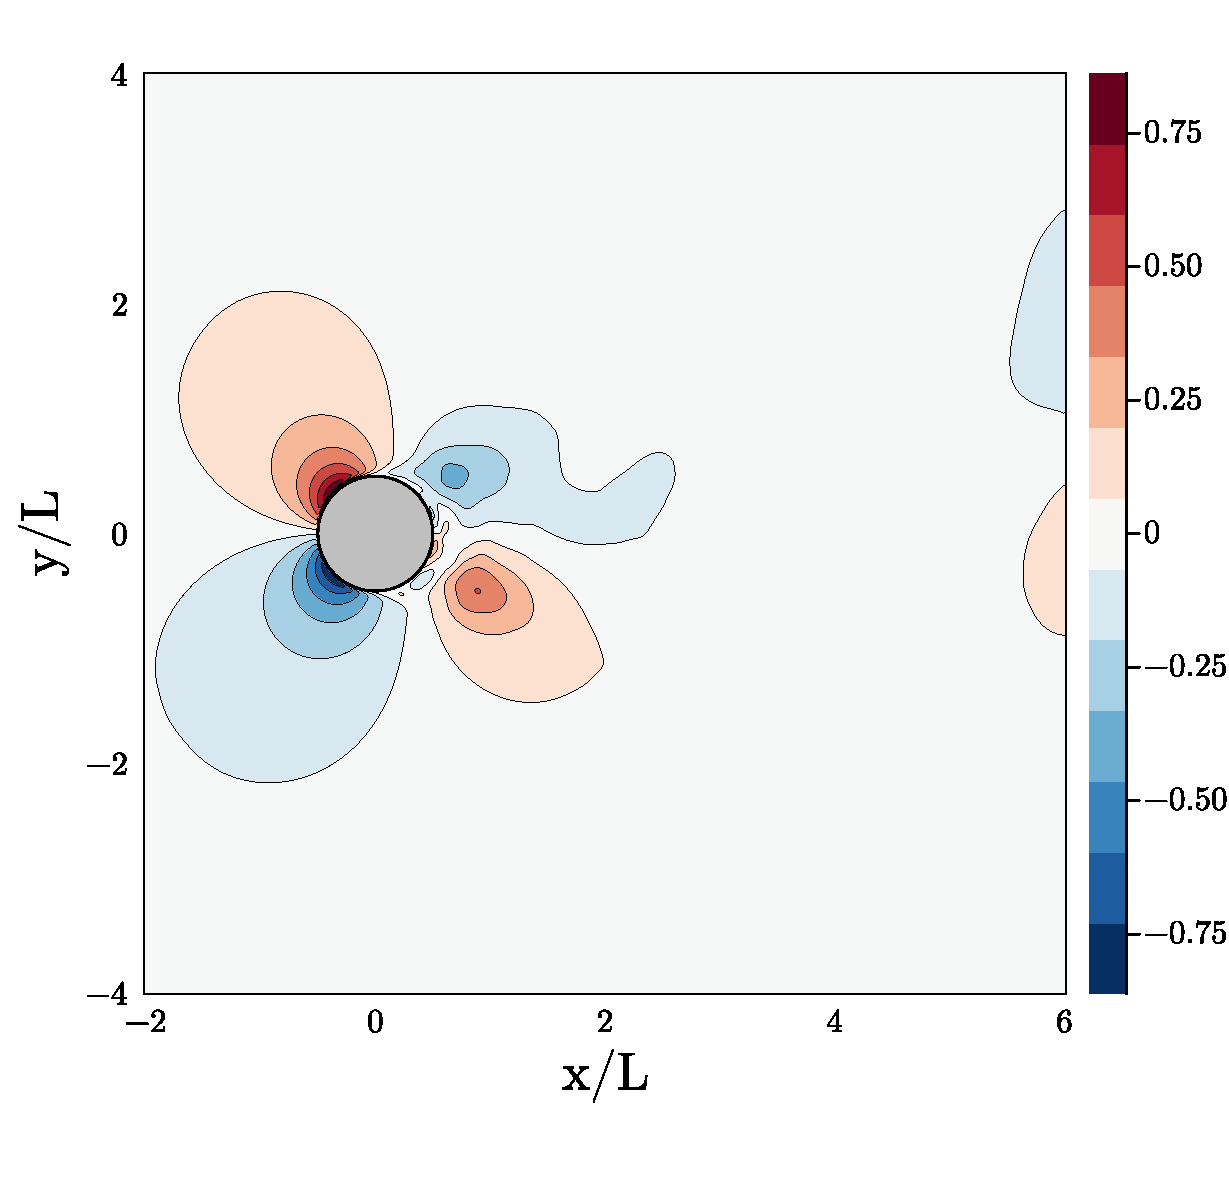
\includegraphics[width=\linewidth]{figures/Results/RE5000/meanflow_panels/meanflow_v_reference.pdf}
    \caption{}
    \label{fig: RE5000_ref_mean_v}
  \end{subfigure}\hfill
  \begin{subfigure}[t]{0.32\textwidth}
    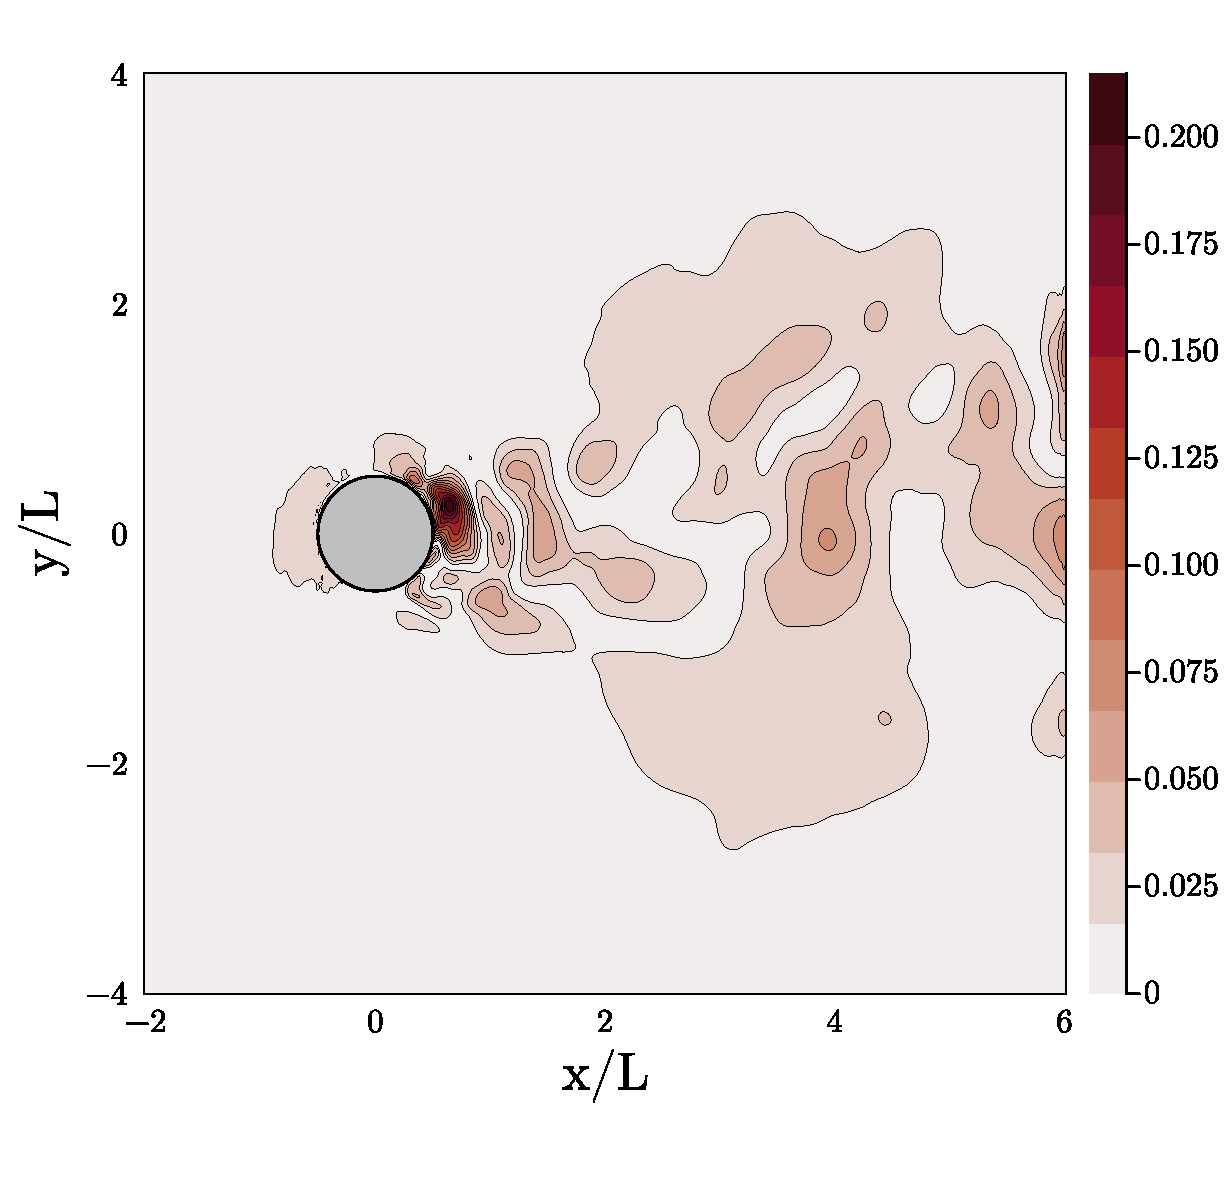
\includegraphics[width=\linewidth]{figures/Results/RE5000/meanflow_panels/meanflow_v_abserror.pdf}
    \caption{}
    \label{fig: RE5000_diff_mean_v}
  \end{subfigure}
\caption{Time-averaged velocity components at $Re=5000$: $\langle u\rangle$ (top) and $\langle v\rangle$ (bottom). Columns: hybrid $\mathcal{S}$, reference $\mathcal{S}_\text{ref}$, and absolute difference $\bigl|\mathcal{S}-\mathcal{S}_\text{ref}\bigr|$. The dominant discrepancy is a coherent band along the wake centreline in $\langle u\rangle$. Lengths scaled by $L$, velocities by $U$.}
\label{fig: RE5000_meanflow}
\end{figure}